\documentclass[12pt]{jarticle}
\usepackage[dvipdfmx]{graphicx}
\usepackage{url}
\usepackage{listings,jlisting}
\usepackage{ascmac}
\usepackage{amsmath,amssymb}

%ここからソースコードの表示に関する設定
\lstset{
  basicstyle={\ttfamily},
  identifierstyle={\small},
  commentstyle={\smallitshape},
  keywordstyle={\small\bfseries},
  ndkeywordstyle={\small},
  stringstyle={\small\ttfamily},
  frame={tb},
  breaklines=true,
  columns=[l]{fullflexible},
  numbers=left,
  xrightmargin=0zw,
  xleftmargin=3zw,
  numberstyle={\scriptsize},
  stepnumber=1,
  numbersep=1zw,
  lineskip=-0.5ex
}
%ここまでソースコードの表示に関する設定

\title{知能プログラミング演習II 課題5}
\author{グループ8\\
  29114003 青山周平\\
}
\date{2020年1月6日}

\begin{document}
\maketitle

\paragraph{提出物} work6
\paragraph{グループ} グループ8
\paragraph{メンバー}
\begin{tabular}{|c|c|c|}
  \hline
  学生番号&氏名&貢献度比率\\
  \hline\hline
  29114003&青山周平&20\\
  \hline
  29114060&後藤拓也&20\\
  \hline
  29114116&増田大輝&20\\
  \hline
  29114142&湯浅範子&20\\
  \hline
  29119016&小中祐希&20\\
  \hline
\end{tabular}

\section{課題の説明}
\begin{description}
\item[必須課題6-1] 課題5にやり残した発展課題があれば参考にして拡張しても良いし,全く新しい独自仕様を考案しても構わない.自由に拡張するか,あるいはもし残っていた問題点があれば完成度を高めよ.
\end{description}

\section{必須課題6-1}
\begin{screen}
課題5にやり残した発展課題があれば参考にして拡張しても良いし,全く新しい独自仕様を考案しても構わない.自由に拡張するか,あるいはもし残っていた問題点があれば完成度を高めよ.
\end{screen}
私の担当箇所は,発展課題5-7に対してUnityを用いて実装したプログラムの,GUI改善やプランニングへの機能追加である.

\subsection{手法}
発展課題5-7では,ブロックワールドにおけるプランニングを実現するための過程として,以下のような実装を行った.
\begin{enumerate}
\item 空間やプランに関するオブジェクトの生成.
\item プランニングを行うための,オブジェクトの動作等に関するスクリプトの作成.
\end{enumerate}

これに引き続いて今回は,ブロックワールドにおけるプランニングを実現するために,以下のような方針を立てた.
\begin{enumerate}
\item プランに用いるブロックをより正確に生成できるようにする.
\item ブロックの管理を容易にする.
\item プランニングの情報を可視化する.
\end{enumerate}

1.に関して,GUIを画面上に表示することで,ブロックを名前や色,形を指定した上で生成できるような仕様とした.

2.に関して,オブジェクトの情報を一覧で表示して生成したオブジェクトの管理を視覚的に行えるような仕様とした.また,フォーカスしているブロックを視覚的に確認できるように,選択中のオブジェクトのアウトラインが表示されるような仕様とした.

3.に関して,2.で作成する一覧と連動して,選択したブロックの情報が画面左下のステータスバーで確認できるようにした.

\subsection{実装}
発展課題5-7で作ったオブジェクトは以下のとおりである.
\begin{description}
\item[Main Camera] 主カメラに関するオブジェクト.Room全体をやや見下ろし気味に映す.
\item[Directional Light] オブジェクト全体を照らす照明.
\item[Master] スクリプトをアタッチするための空オブジェクト.
\item[Room] 6個のPlaneオブジェクトを子に持つ,立方体の部屋を構成するオブジェクト.
\item[Cube] 直方体のブロックを生成するプレハブ.
\item[Sphere] 球のブロックを生成するプレハブ.
\item[Torus] 円環体のブロックを生成するプレハブ.
\end{description} 

新しく作った主なオブジェクトは以下のとおりである.
\begin{description}
\item[EventSystem] GUIにおいてButtonやInputFieldを機能させるための,フォーカス情報等を掌るオブジェクト.
\item[Canvas] Generator,Preparator,Staterを子オブジェクトに持つ,GUIの大元となるオブジェクト.
\item[Generator] オブジェクトを生成するためのパネル.子オブジェクトにInputFieldName,DropdownColor,DropdownShape,ButtonGenを持つ.
\item[Preparator] 生成したオブジェクトの一覧を管理するパネル.子オブジェクトにScrollView,ButtonRm,ButtonPlanningを持つ.
\item[Stater] オブジェクトの情報等を表示するためのパネル.子オブジェクトにTextStatus,Scrollbarを持つ.
\item[ListObj] PreparatorにおけるScrollViewの要素となるプレハブ.
\end{description} 

C\#スクリプトでは以下のものが実装されている.
\begin{description}
\item[Clicked] クリックされたオブジェクトにフォーカスを当てるスクリプト.Masterにアタッチされる.
\item[Operationg] Clickedでフォーカスされたオブジェクトにキーボード入力を反映するスクリプト.Masterにアタッチされる.
\item[Generator] Generatorオブジェクトで得た情報に合わせて,ブロックを生成するスクリプト.ButtonGenにアタッチされる.
\item[Destroyer] Preparatorオブジェクトで選択されたブロックを削除するためのスクリプト.ButtonRmにアタッチされる.
\item[Manager] ListObjプレハブにアタッチされる,各インスタンスが1対1で対応するブロックを保持するためのスクリプト.
\item[SelectOnList] ListObjプレハブにアタッチされる,インスタンスが自身にアウトラインや削除のフォーカスを当てるためのスクリプト.
\item[Starter] GUIの一部を非表示にし,プランニングを開始するためのスクリプト.ButtonPlanningにアタッチされる.
\item[CollisionGetter] 自身と衝突中のブロックを保持するスクリプト.各ブロックにアタッチされる.
\item[StateGetter] SelectOnListでフォーカスされたブロックと衝突中のブロックをStaterに表示するスクリプト.Masterにアタッチされる.
\end{description}

\subsubsection{プランに用いるオブジェクトをより正確に生成できるようにする.}
Unity\cite{unity}においてGUIを作成するために,Unityの標準機能に含まれるuGUI\cite{ugui}を用いた.

まず,GUI制作をUnity上で開始するために,Canvasオブジェクトを生成した.Canvasオブジェクトは実行環境によって,そのサイズが動的に変化するため,シーンビューにおける大きさは意味を持たない.その仕様を理解するまでは扱いに戸惑った.

次に,ブロック生成のためのGUIであるGeneratorオブジェクト(図\ref{fig:an1})を作るために,GeneratorオブジェクトにはPanelを,名前を入力するためのフォーム(InputFieldName)にはInputFieldを,色や形の選択(DropdownColor,DropdownShape)にはDropdownを,生成ボタン(ButtonGen)にはButtonをそれぞれ用いた.これらUIに関するパーツはいずれもRectTransformコンポーネントを用いて配置される.

RectTransformの特徴として,アンカーとピボットが挙げられる.これらはブロック等のオブジェクトの座標指定で用いられるTransformコンポーネントには含まれない.今回ピボットは用いなかったが,アンカーはGUIパーツの配置を行う上では欠かせないものであることが分かった.

アンカーは,指定した位置を基準として,オブジェクトの相対座標を指定するものである.図\ref{fig:an1}に示すように,Canvasの右上部である位置に表示されている4つの三角がアンカーの基準点を示すものであり,パネルはアンカーから左下部に相対座標で配置されている.これにより,実行環境により画面サイズが変化しても,図\ref{fig:an2}や図\ref{fig:an3}で示すようにレイアウトを崩さずに表示されることが確認できる.

\begin{figure}[!hbt]
  \begin{center}
    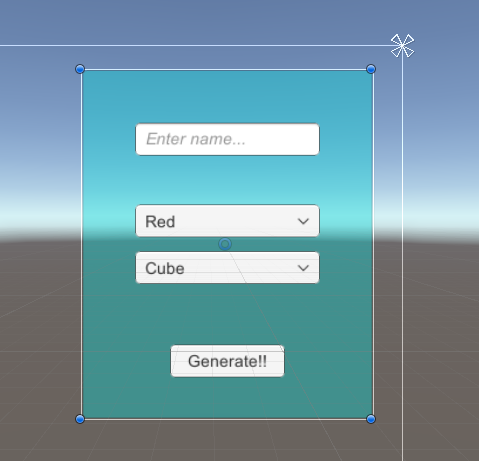
\includegraphics[scale=0.5]{images/BWP_Work6/anchor1.png}
  \end{center}
  \caption{Generatorオブジェクト}
  \label{fig:an1}
\end{figure}

\begin{figure}[!hbt]
  \begin{center}
    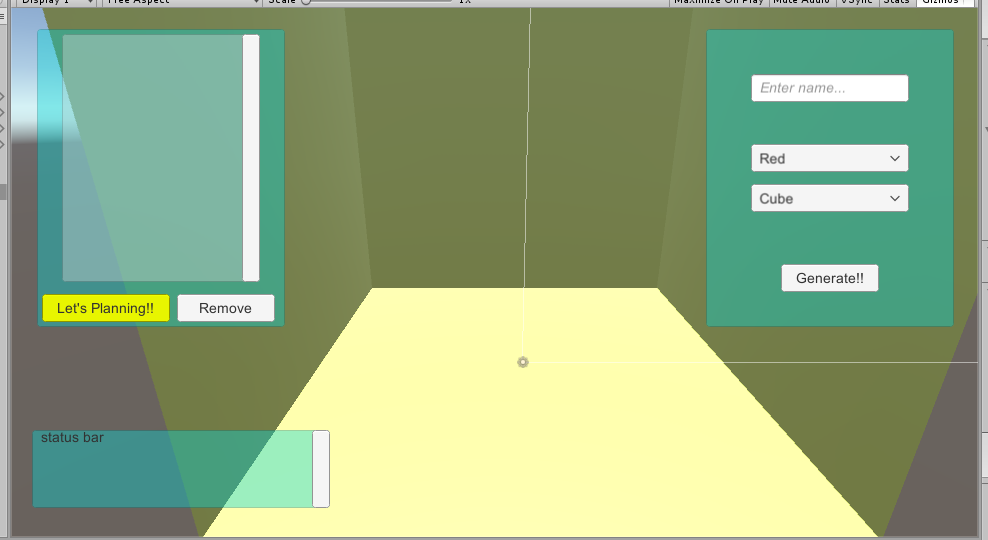
\includegraphics[scale=0.5]{images/BWP_Work6/anchor2.png}
  \end{center}
  \caption{横長の画面における表示}
  \label{fig:an2}
\end{figure}

\begin{figure}[!hbt]
  \begin{center}
    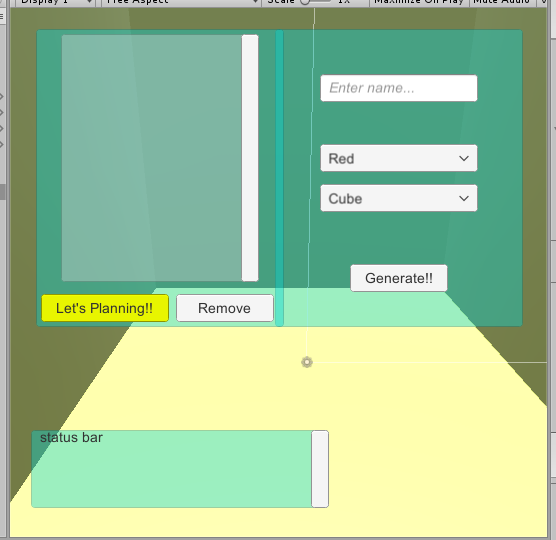
\includegraphics[scale=0.5]{images/BWP_Work6/anchor3.png}
  \end{center}
  \caption{縦長の画面における表示}
  \label{fig:an3}
\end{figure}

\clearpage

次に,配置したGenerator内のオブジェクトを用いて,ブロックを生成するためのスクリプト(Generator.cs)を生成する.
ブロックはソースコード\ref{src:gen}で示すように生成される.

\begin{lstlisting}[caption=Generatorクラス, label=src:gen]
public class Generator : MonoBehaviour
{
    ...
    public void Generate()
    {
        ...
        GameObject obj = (GameObject)Resources.Load("Cube");
        switch (ddShape.value)
        {
            case 0:
                obj = (GameObject)Resources.Load("Cube");
                break;
            case 1:
                obj = (GameObject)Resources.Load("Sphere");
                break;
            case 2:
                obj = (GameObject)Resources.Load("Torus");
                break;
        }
        GameObject target = Instantiate(obj, obj.transform.position, Quaternion.identity);
        target.name = name;
        target.GetComponent<Renderer>().material.color = getColor(ddColor.value).color;

        GameObject _text = Instantiate(textPrefab, content.transform);
        _text.GetComponentInChildren<Text>().text = name;
        _text.GetComponent<Manager>().planObj = target;
    }
    
    ...

    Material getColor(int num)
    {
        Material color = matR;
        switch(num)
        {
            case 0:
                color = matR;
                break;
            case 1:
                color = matG;
                break;
            case 2:
                color = matB;
                break;
        }
        return color;
    }
}
\end{lstlisting}

ddShape.valueを介してDropdownShapeで選択された形を選択し,Resource.Loadメソッドでプレハブを取得している.取得したプレハブをInstantiateメソッドで生成し,生成したインスタンスの名前をInputFieldNameで入力した名前に書き換え,色をddColor.valueを介してDropdownShapeで選択された色に書き換えている.

このスクリプトをButtonGenにアタッチすることで,ボタンをクリックしたときにこのスクリプトは呼び出され,実行される.
\clearpage

\subsubsection{ブロックの管理を容易にする.}
ブロックを管理するためのGUIであるPreparatorオブジェクト(図\ref{fig:pre})を作るために,PreparatorオブジェクトにはPanelを,ブロックを表示するリスト(ScrollView)にはScrollViewを,リスト内の要素(ListObj)にはButtonをプレハブ化したもの,リスト内の要素削除ボタン(ButtonRm)とプランニング開始ボタン(ButtonPlanning)にはButtonをそれぞれ用いた.

\begin{figure}[!hbt]
  \begin{center}
    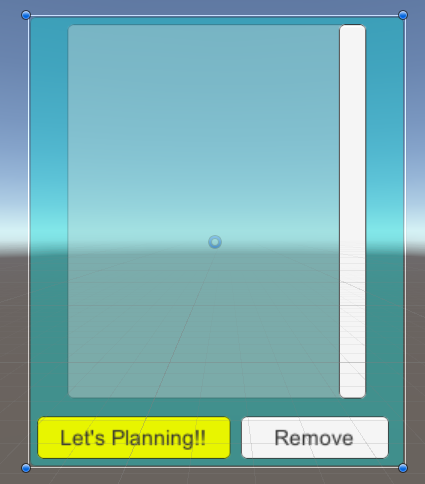
\includegraphics[scale=0.5]{images/BWP_Work6/preparator.png}
  \end{center}
  \caption{Preparatorオブジェクト}
  \label{fig:pre}
\end{figure}

ScrollViewを作成する\cite{sv}にあたり,ListObjは要素の選択を可能にするために,Buttonを用いて実装した.

Generatorスクリプト(ソースコード\ref{src:gen})の変数\_textによって,ListObjからインスタンスが生成されている.この際,スクロールバーに表示するためには適切な位置の子オブジェクトとして格納する必要がある.これは,Instantiateの引数に親オブジェクトのtransformを渡すことで実現した.
また,ここで生成したインスタンスに,先程生成したブロックのインスタンスへの参照も,Managerスクリプトの変数を介して渡している.これにより,ListObjのインスタンスから対応するブロックへのアクセスを可能としている. \\

次に,ScrollViewから選択した要素にアウトラインを付けるためのスクリプトSelectOnList,StateGetterを実装する.

まず,アウトラインはUnityの標準機能に備わっていないため,アセットQuickOutline\cite{outline}を導入し,各ブロックに非アクティブ状態でアタッチした.

その上で,引数で渡されたブロックのアウトラインをアクティブにするStateGetterクラス内のFocusOutlineメソッドを,ソースコード\ref{src:outline}に示す.

\begin{lstlisting}[caption=StateGetterクラス内のFocusOutlineメソッド, label=src:outline]
    public GameObject target;
    
    public void FocusOutline (GameObject newObj) {
        if (target != null) {
            target.GetComponent<Outline> ().enabled = false;
        }
        if (newObj != null) {
            newObj.GetComponent<Outline> ().enabled = true;
        }
        target = newObj;
    }
\end{lstlisting}

アウトラインをアクティブにしたブロックをtargetに保持することで,フォーカスが外れた際の非アクティブ化も同時に行えるようになっている.StateGetterはMasterに1つだけアタッチされることで,フォーカスの管理を一元的に行うことを可能とした.

SelectOnListスクリプトは各ListObjインスタンスにアタッチされることで,フォーカスが当てられたときにSelectOnListスクリプトからFocusOutlineメソッドを呼び出すことで,自身にアウトラインを付けることができる.(図\ref{fig:off},\ref{fig:on})

\begin{figure}[!hbt]
  \begin{center}
    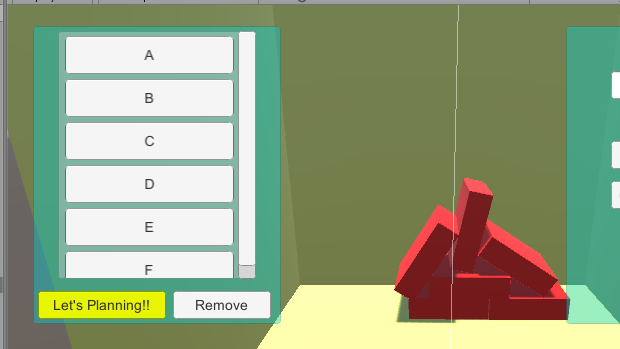
\includegraphics[scale=0.5]{images/BWP_Work6/outline1.png}
  \end{center}
  \caption{非フォーカス時}
  \label{fig:off}
\end{figure}

\begin{figure}[!hbt]
  \begin{center}
    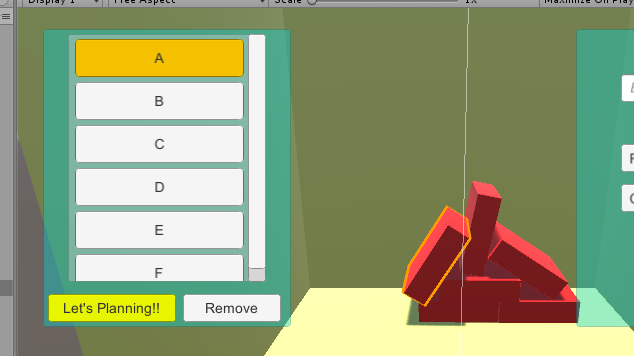
\includegraphics[scale=0.5]{images/BWP_Work6/outline2.png}
  \end{center}
  \caption{フォーカス時}
  \label{fig:on}
\end{figure}
\clearpage

\subsubsection{プランニングの情報を可視化する.}
プランニングの情報表示のためのGUIであるStaterオブジェクト(図\ref{fig:stater})を作るために,StaterオブジェクトにはPanelを,情報を表示するテキスト(TextStatus)にTextを用い,一度に全部を表示できないときのためにScrollbarを作成した\cite{sb}.

\begin{figure}[!hbt]
  \begin{center}
    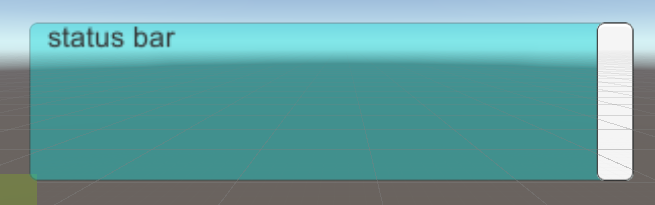
\includegraphics[scale=0.5]{images/BWP_Work6/stater.png}
  \end{center}
  \caption{Staterオブジェクト}
  \label{fig:stater}
\end{figure}

フォーカスされたオブジェクトの衝突情報を取得するために,CollisionGetterスクリプトを作成し,各ブロックにアタッチした.それをソースコード\ref{src:collision}に示す.

\begin{lstlisting}[caption=CollisionGetterクラス, label=src:collision]
public class CollisionGetter : MonoBehaviour {

    public List<GameObject> colList;

    void Awake () {
        colList = new List<GameObject> ();
    }

    void OnCollisionStay (Collision collision) {
        if (!colList.Contains(collision.gameObject)) {
            colList.Add (collision.gameObject);
        }
    }
    void OnCollisionExit (Collision collision) {
        colList.Remove (collision.gameObject);
    }
}
\end{lstlisting}

衝突相手のブロック名がcolListに1つだけ格納される.この際,同じブロックに対して複数の衝突判定を持つときにcolListに複数同じ要素が含まれないようにするために,要素の追加はOnCollisionEnterメソッドではなくOnCollisionStayメソッドを用いて常に監視することで,colListの要素が常に正確になるような実装をした.

このリストをStateGetterから取得し,Staterに反映することで,フォーカスしたブロックの衝突判定を,常に可視化することを実現した.

\subsection{実行例}
task5-7/build/Block World Planning.exeを起動したところ,図\ref{fig:run0}のような画面が得られる.

\begin{figure}[!hbt]
  	\begin{center}
  		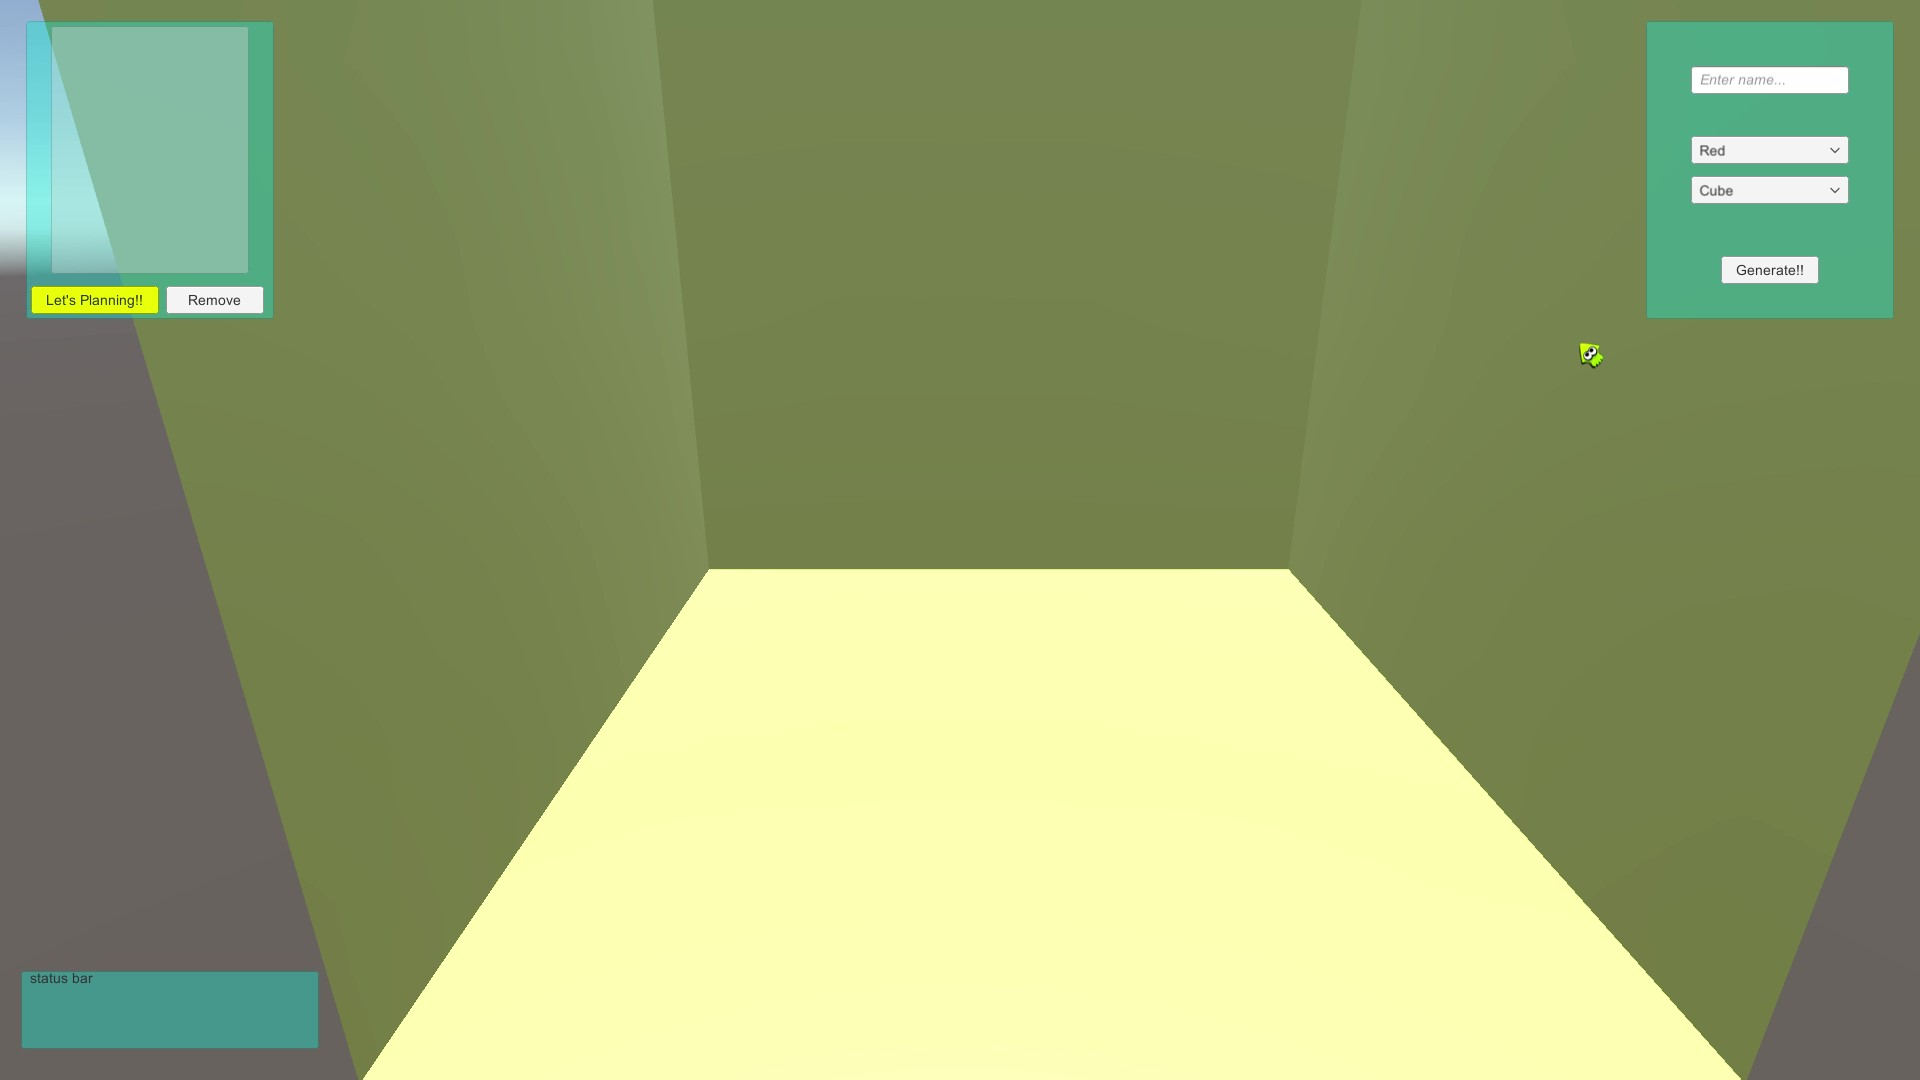
\includegraphics[scale=0.2]{images/BWP_Work6/bwp0.jpg}
	\end{center}
  	\caption{起動時の画面}
  	\label{fig:run0}
\end{figure}
\clearpage

Generatorを用いてブロックを生成すると,Preparatorにも反映されることが分かる(図\ref{fig:run1},\ref{fig:run2}).

\begin{figure}[!hbt]
  	\begin{center}
  		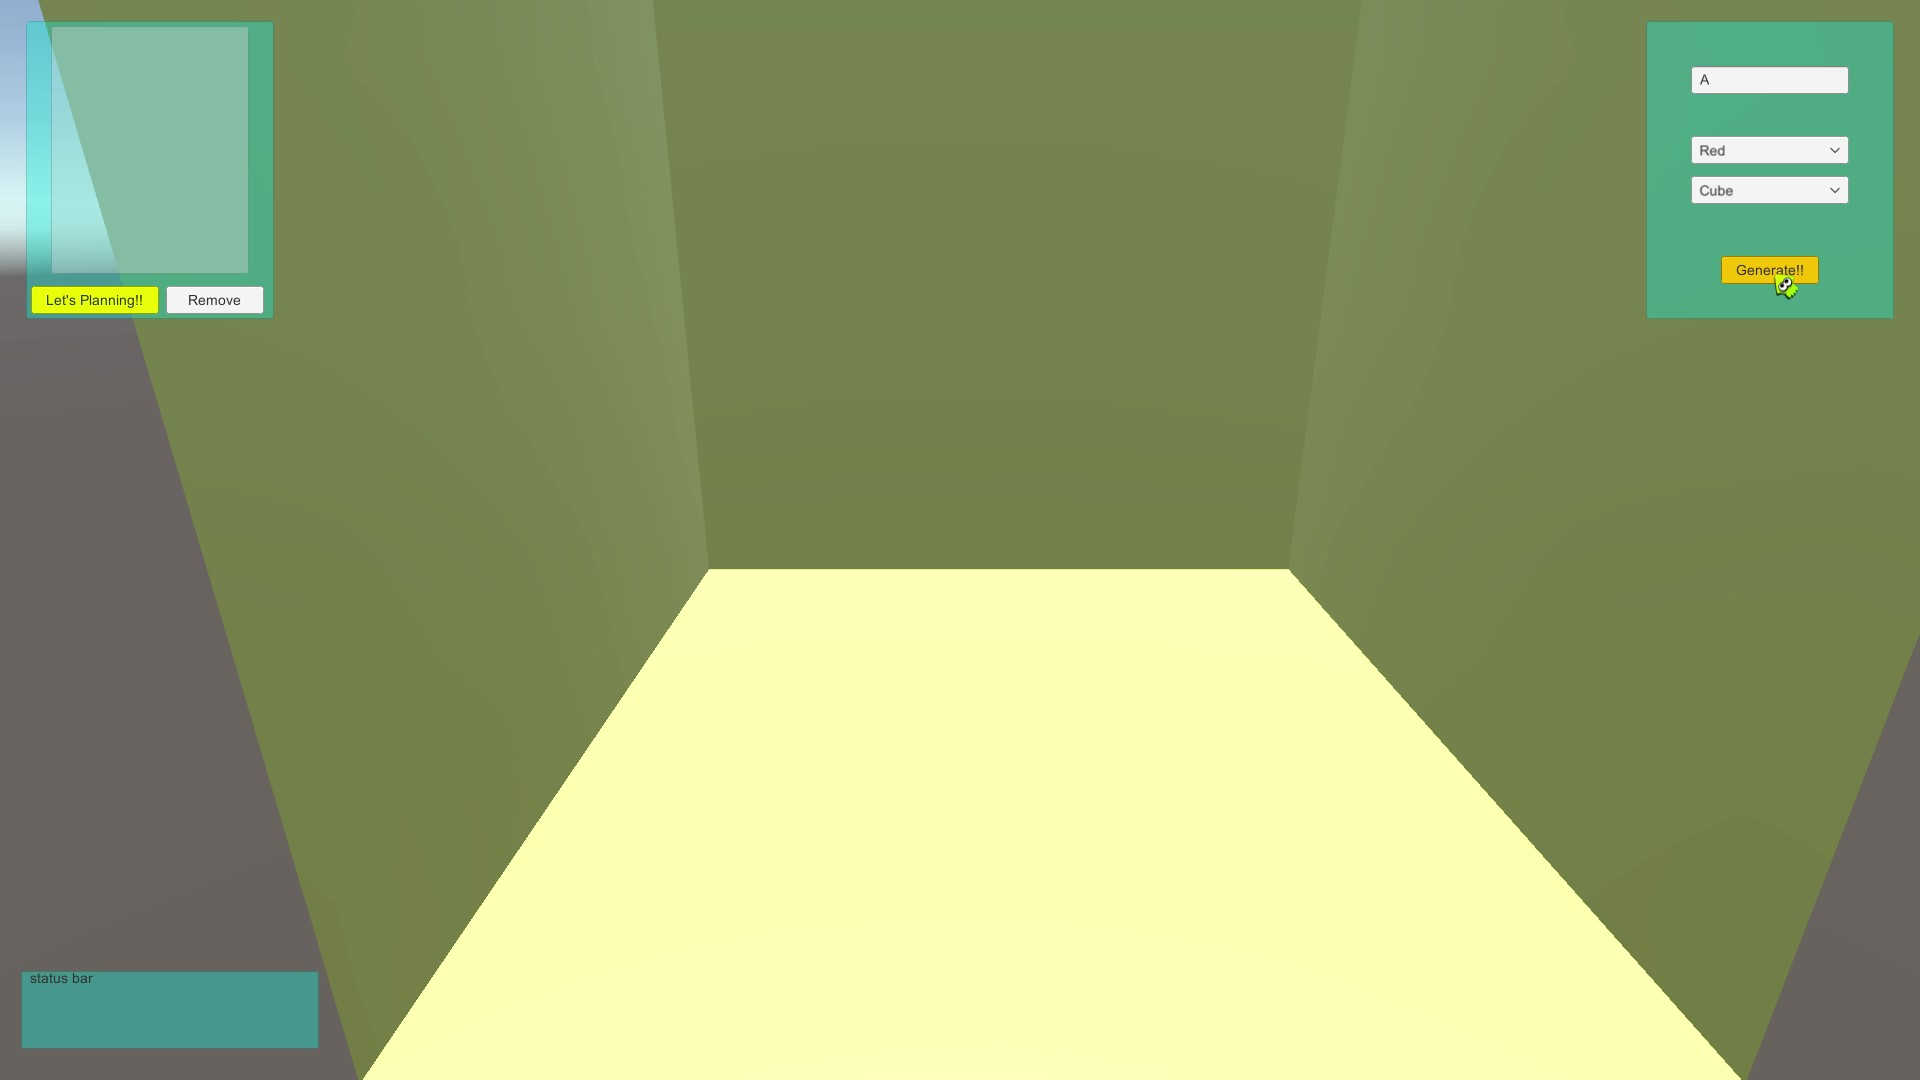
\includegraphics[scale=0.2]{images/BWP_Work6/bwp1.jpg}
  		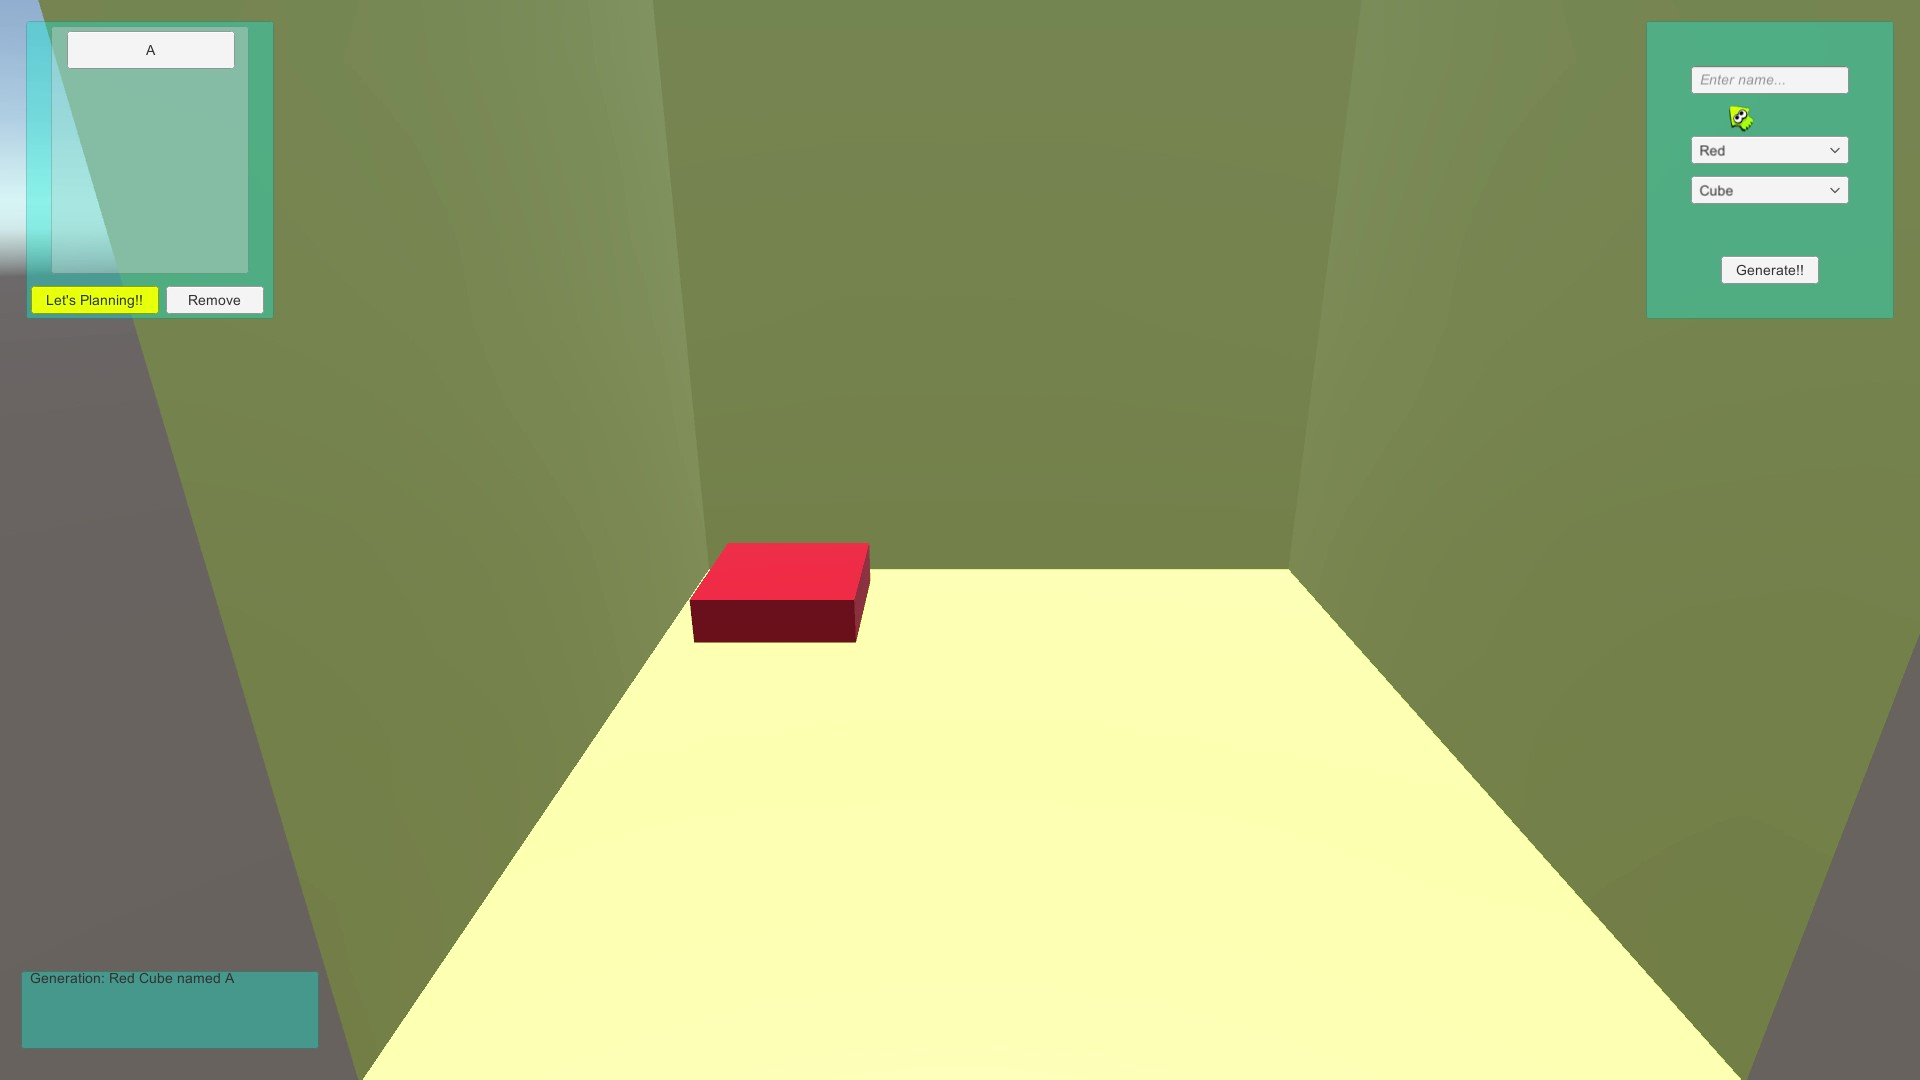
\includegraphics[scale=0.2]{images/BWP_Work6/bwp2.jpg}
	\end{center}
  	\caption{赤い球をAという名前で生成}
  	\label{fig:run1}
\end{figure}

\begin{figure}[!hbt]
  	\begin{center}
  		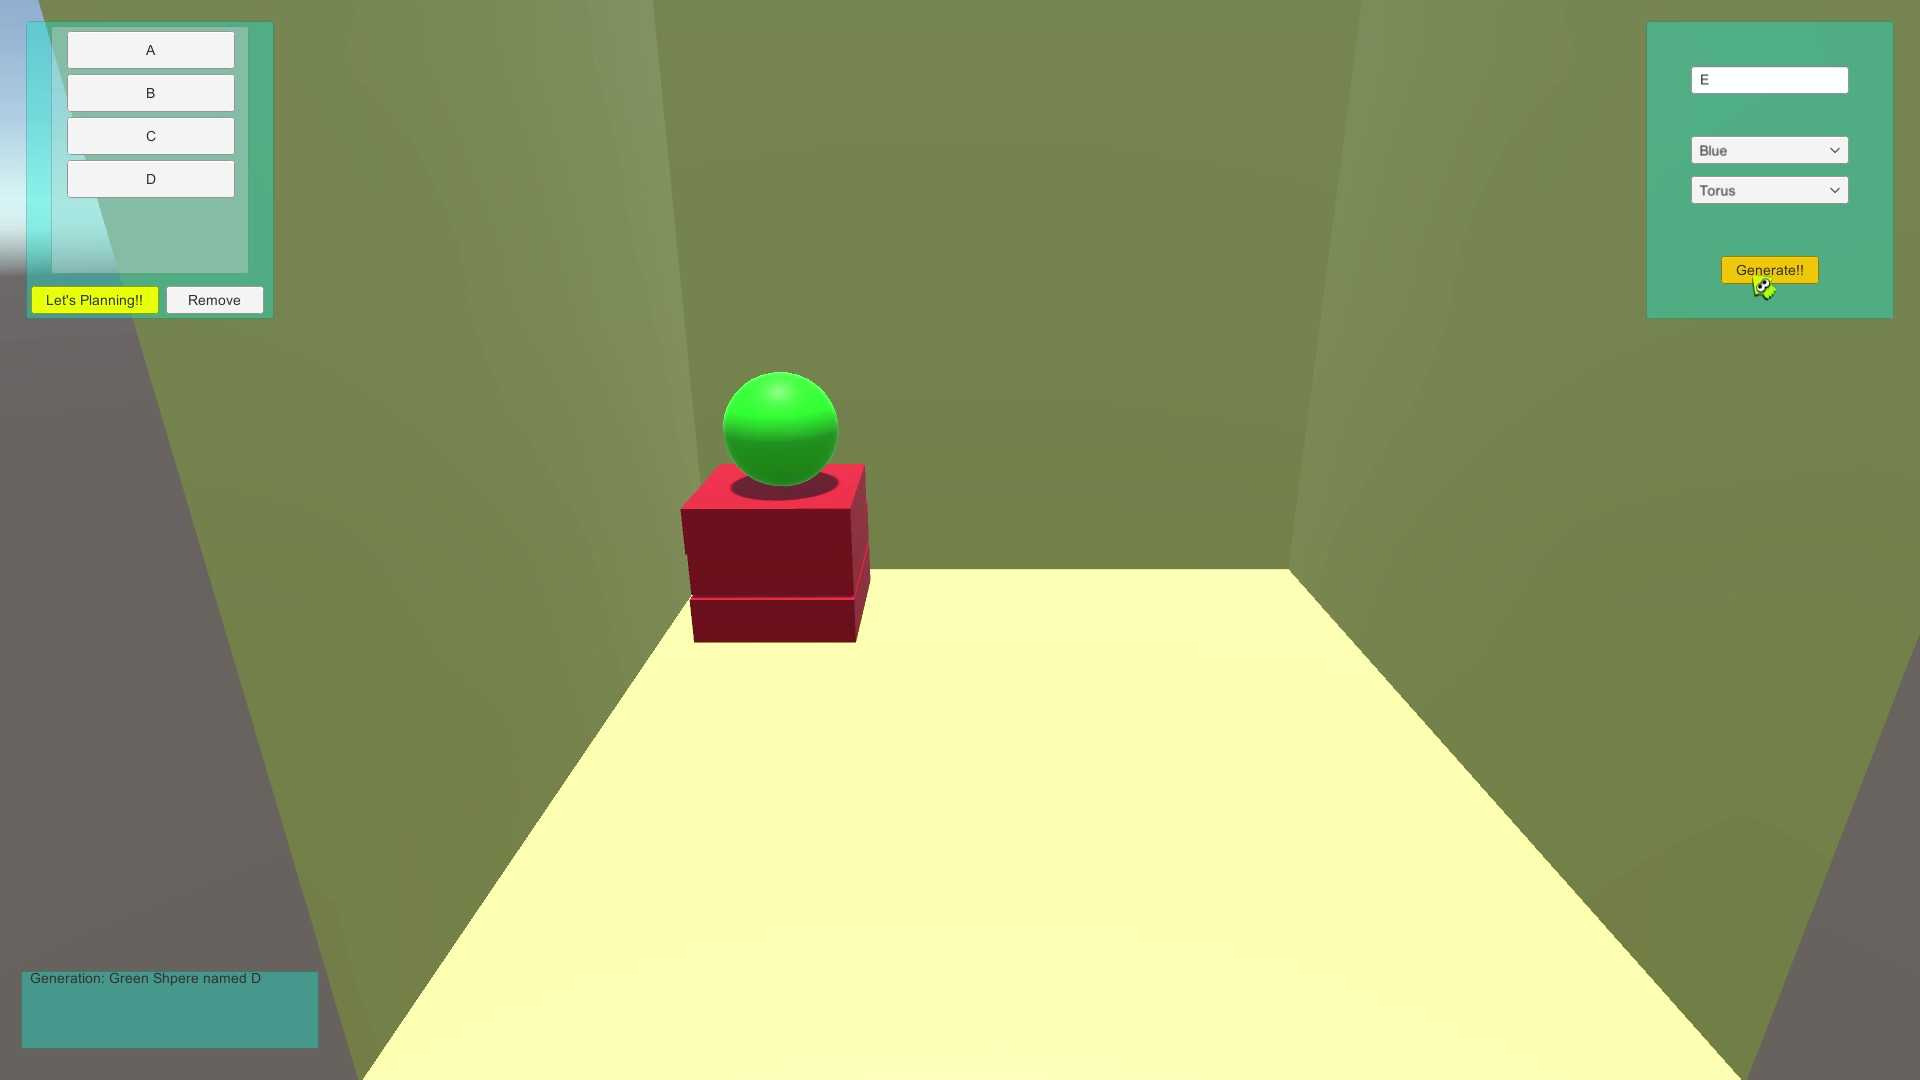
\includegraphics[scale=0.2]{images/BWP_Work6/bwp3.jpg}
  		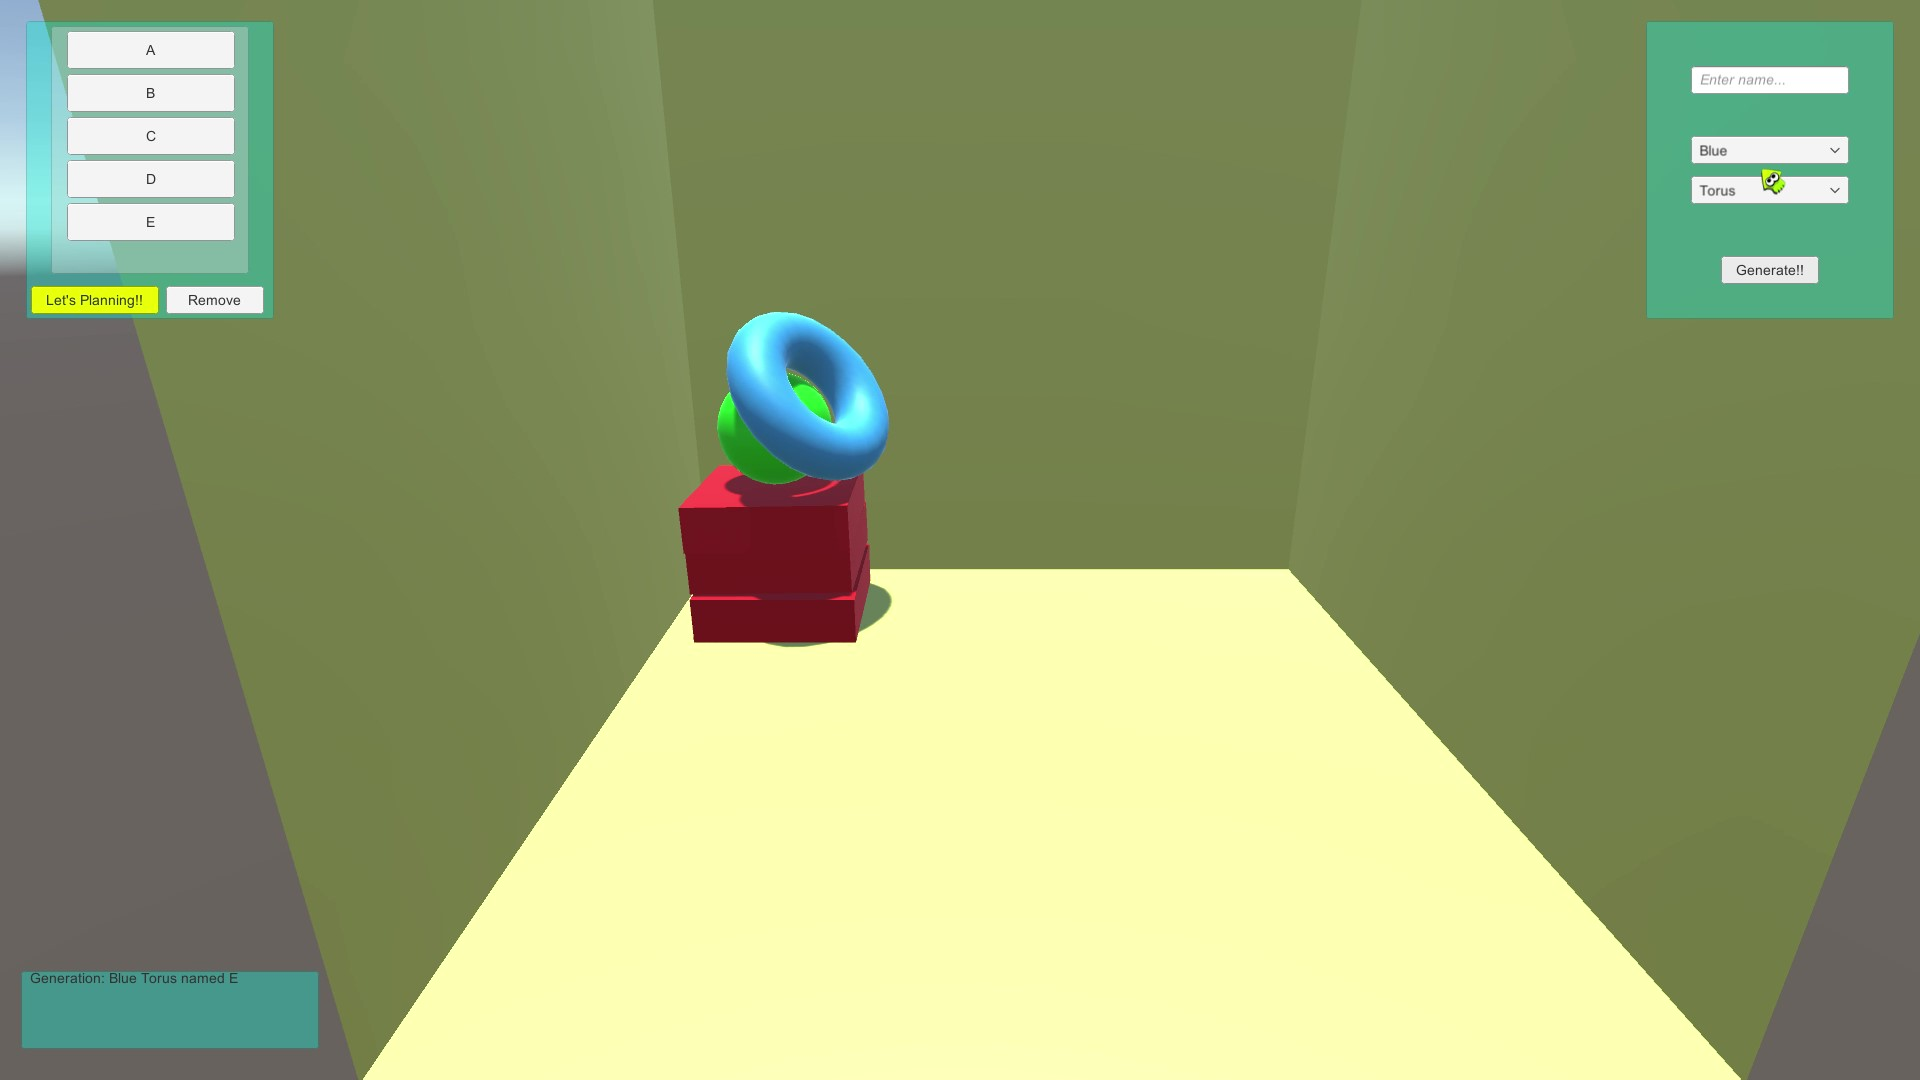
\includegraphics[scale=0.2]{images/BWP_Work6/bwp4.jpg}
	\end{center}
  	\caption{青い円環体をEという名前で生成}
  	\label{fig:run2}
\end{figure}
\clearpage

Preparatorで要素を選択すると,対応するブロックのアウトラインが表示される(図\ref{fig:run3}).

\begin{figure}[!hbt]
  	\begin{center}
  		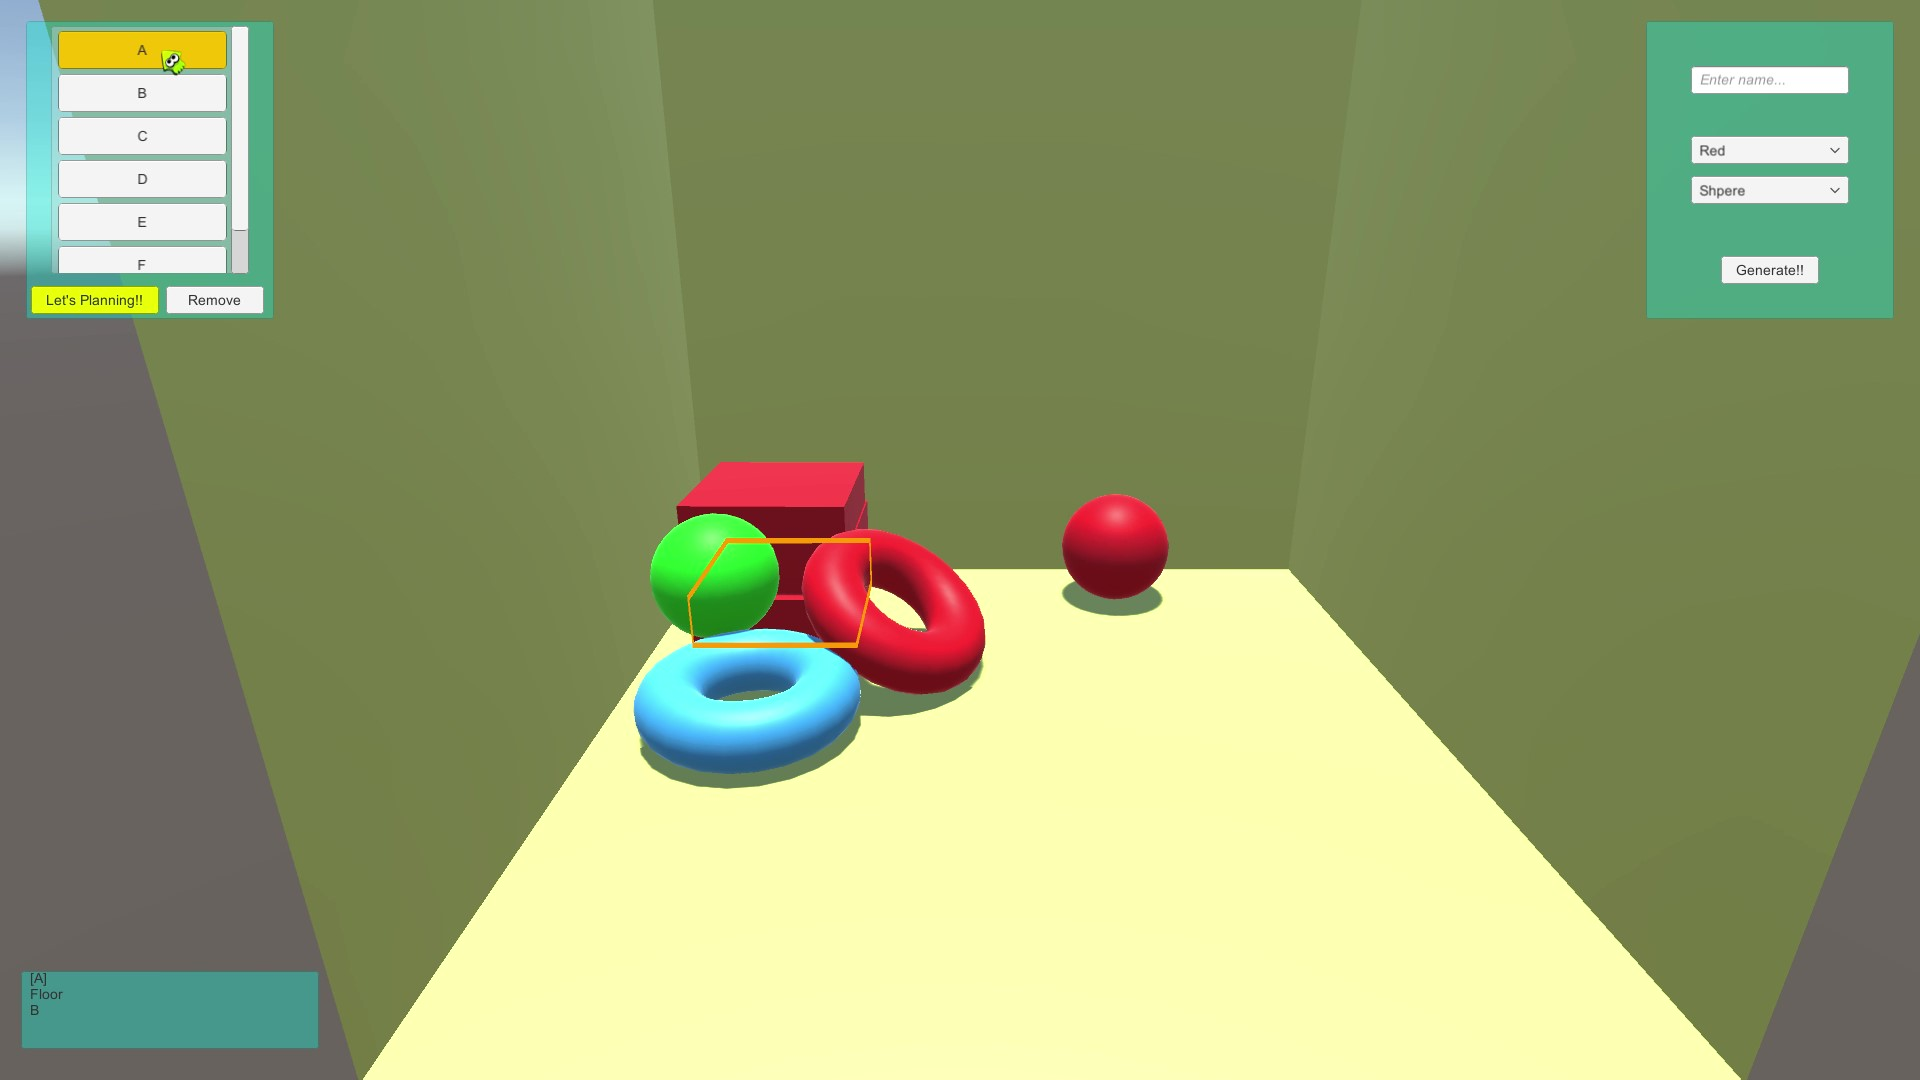
\includegraphics[scale=0.2]{images/BWP_Work6/bwp5.jpg}
	\end{center}
  	\caption{Aにフォーカス}
  	\label{fig:run3}
\end{figure}
\clearpage

フォーカスしたブロックはRemoveボタンで削除できる(図\ref{fig:run4}).

\begin{figure}[!hbt]
  	\begin{center}
  		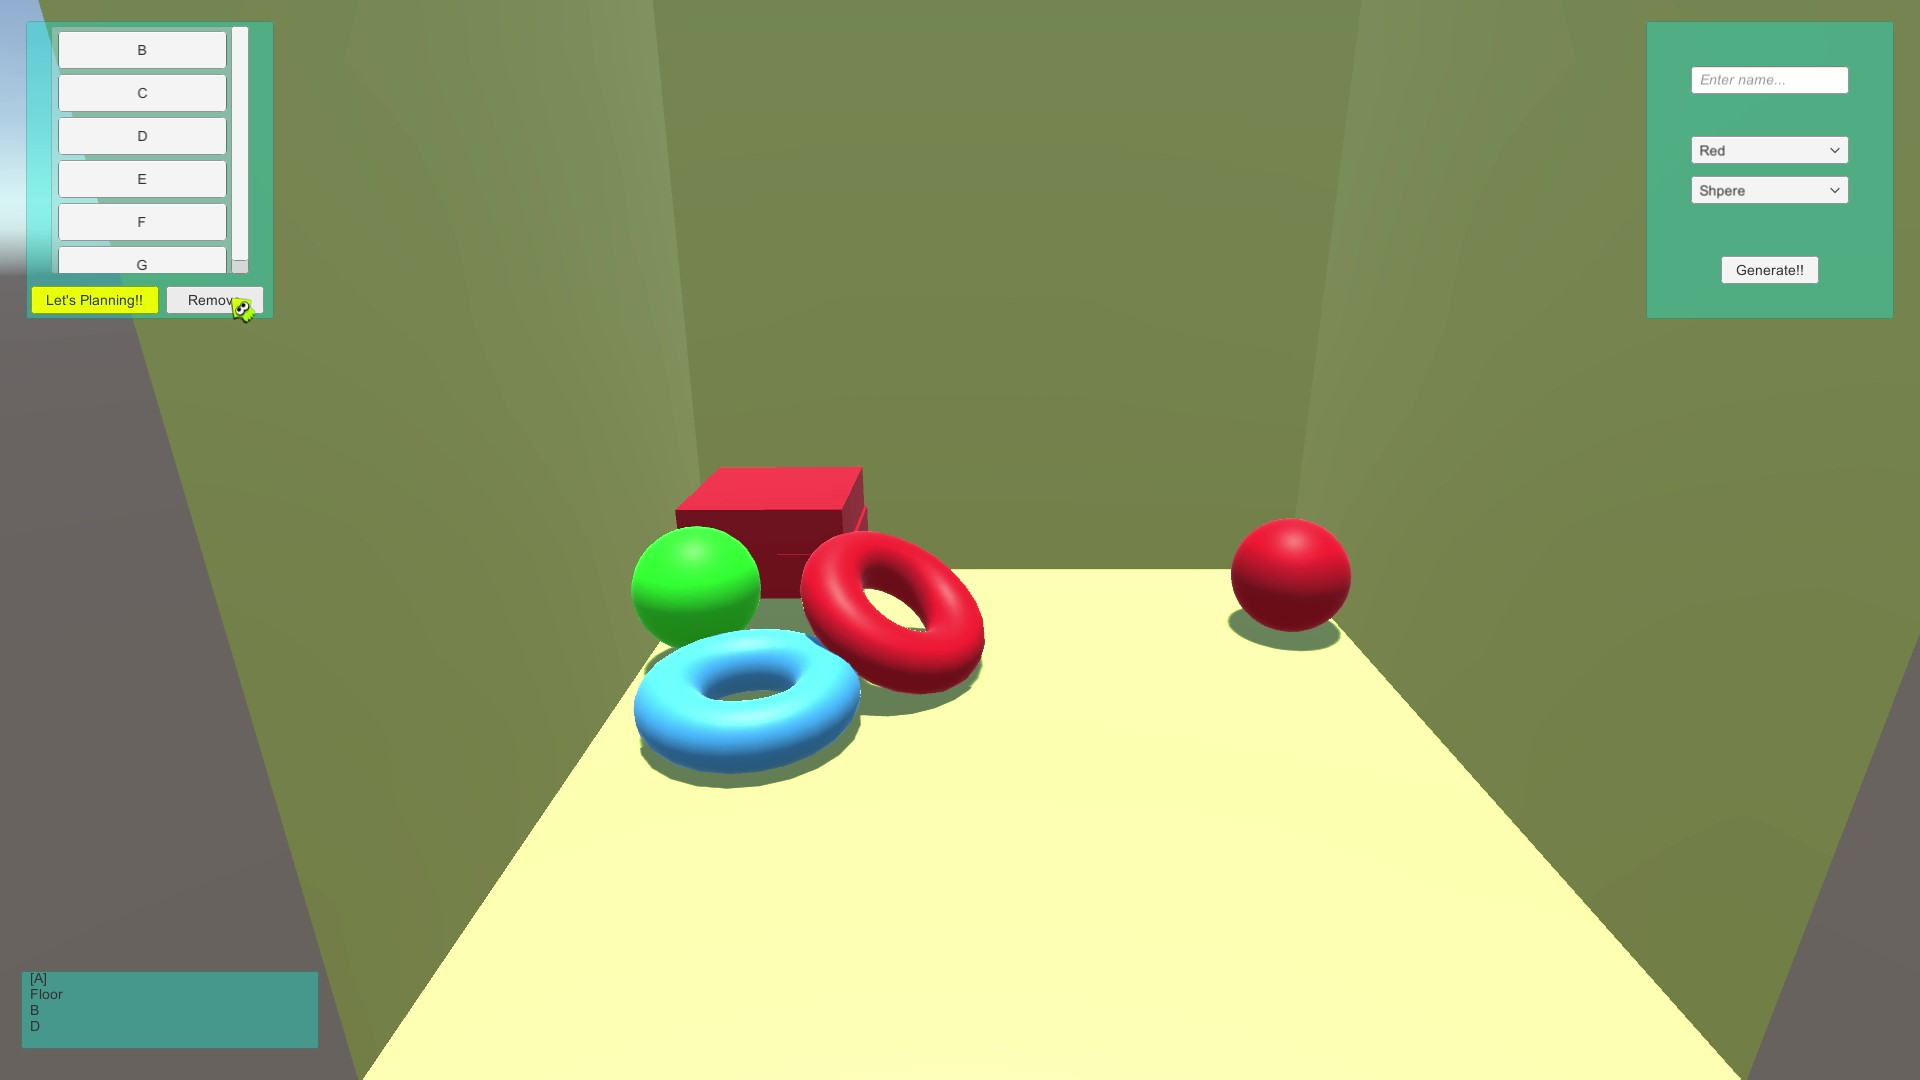
\includegraphics[scale=0.2]{images/BWP_Work6/bwp6.jpg}
	\end{center}
  	\caption{Aを削除}
  	\label{fig:run4}
\end{figure}
\clearpage

ブロックの生成や削除が完了したら,Let's Planningボタンでプランニングを開始する(図\ref{fig:run5}).

\begin{figure}[!hbt]
  	\begin{center}
  		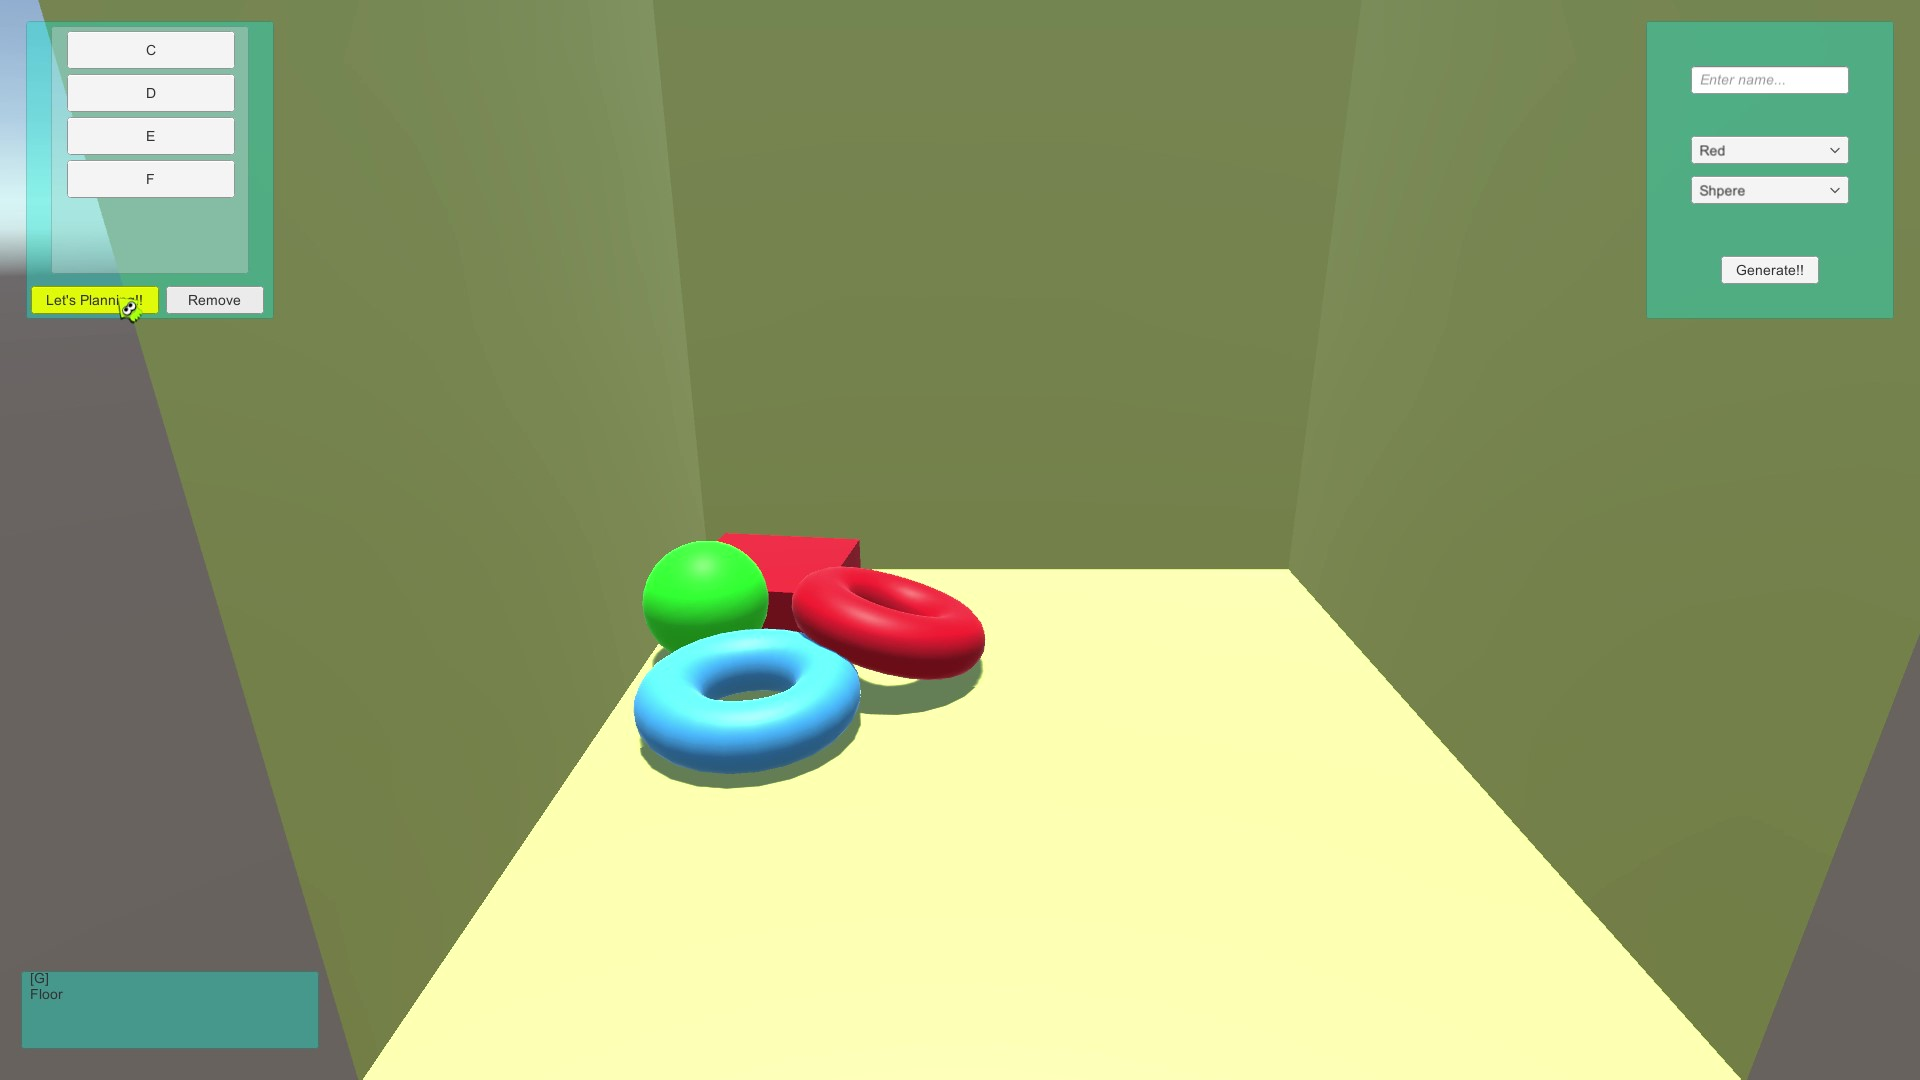
\includegraphics[scale=0.2]{images/BWP_Work6/bwp7.jpg}
	\end{center}
  	\caption{プランニング初期状態}
  	\label{fig:run5}
\end{figure}
\clearpage

フォーカスしたブロックと衝突しているブロックの情報がStaterに表示される(図\ref{fig:run6},\ref{fig:run7}).

\begin{figure}[!hbt]
  	\begin{center}
  		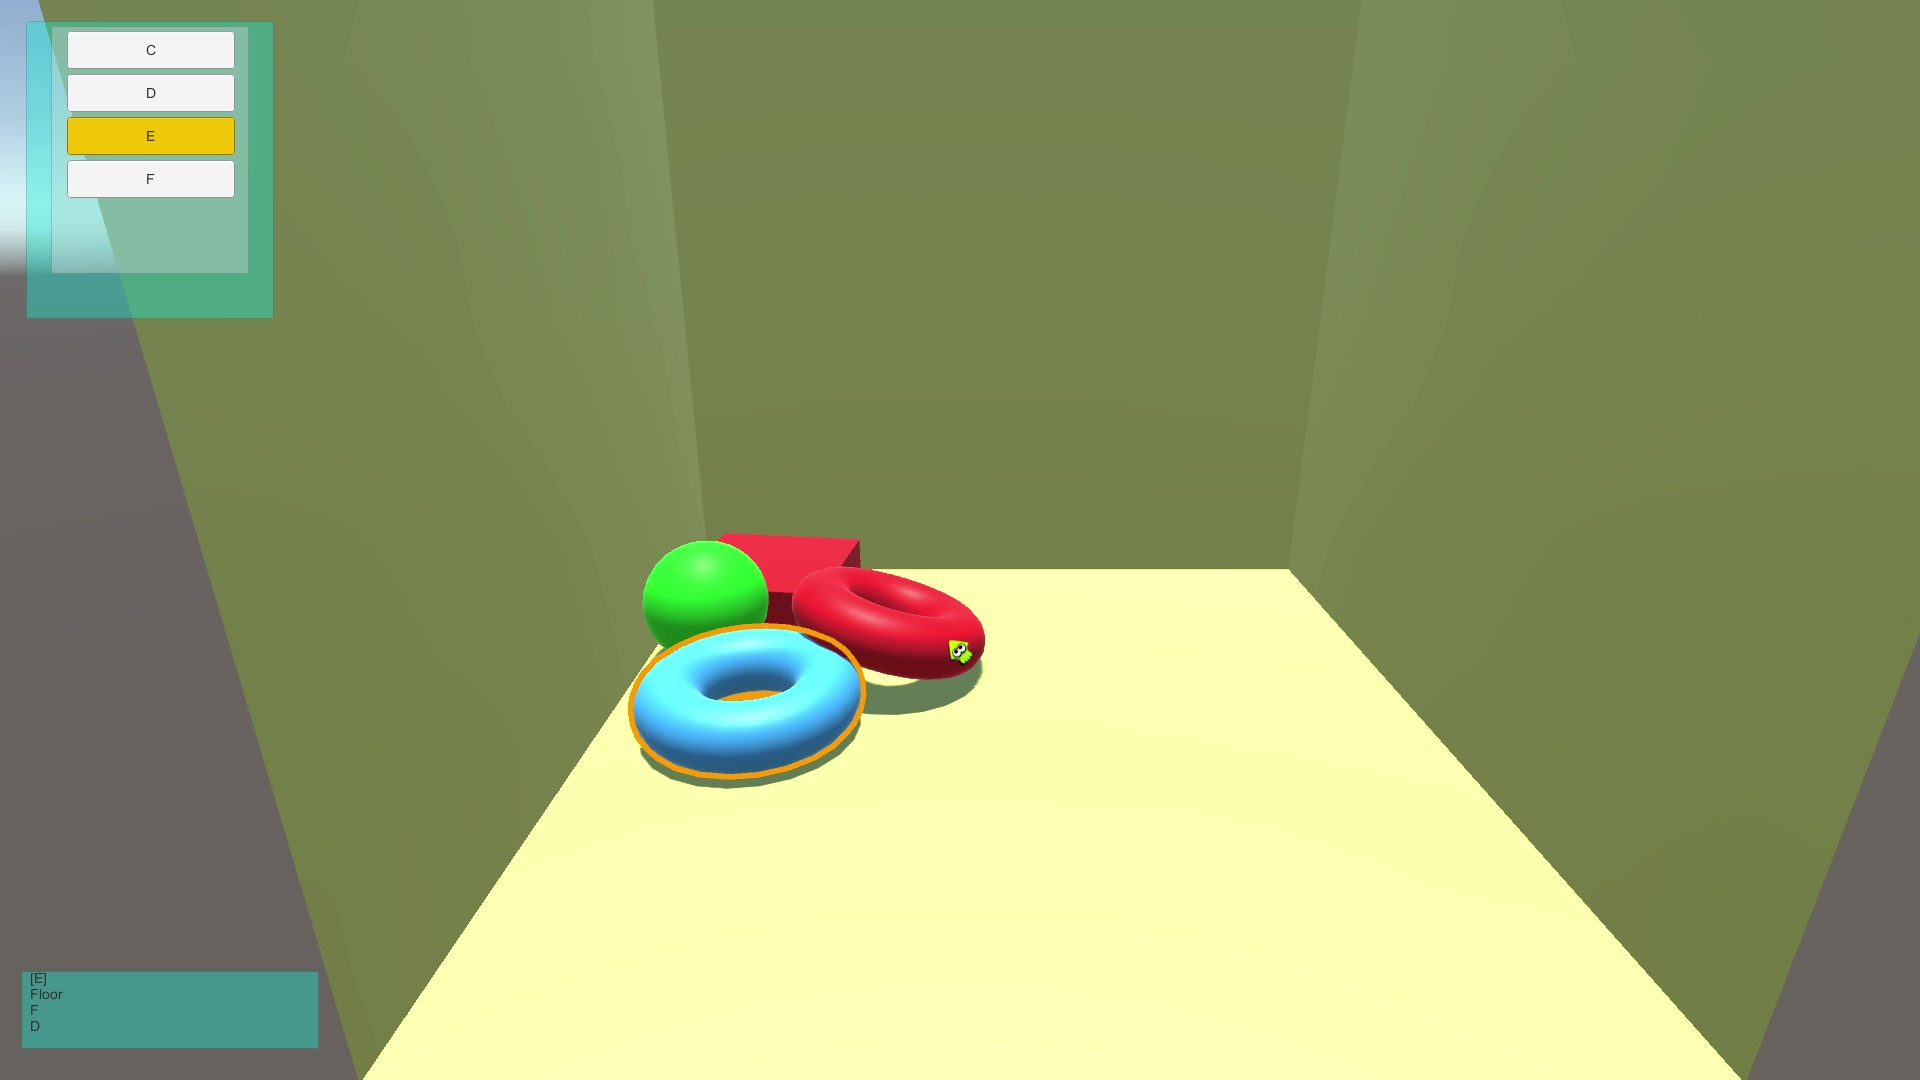
\includegraphics[scale=0.2]{images/BWP_Work6/bwp8.jpg}
  		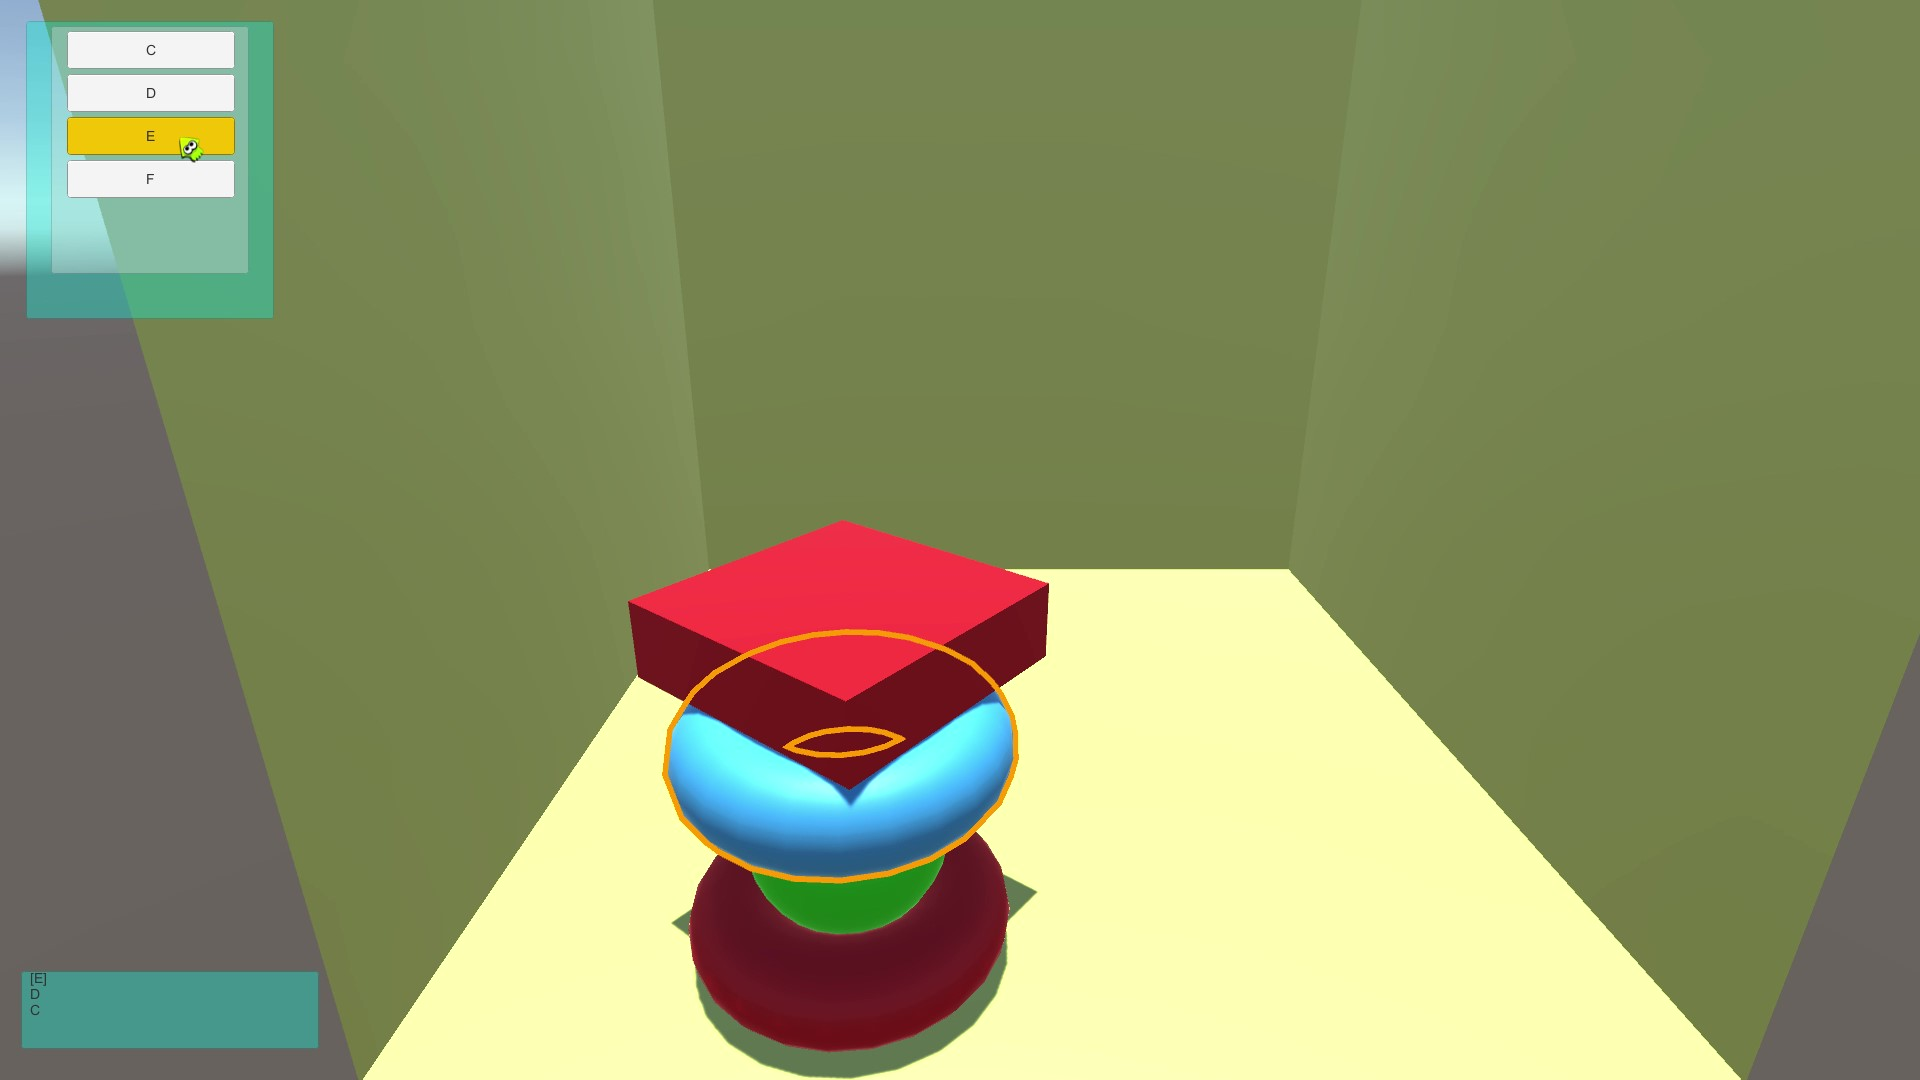
\includegraphics[scale=0.2]{images/BWP_Work6/bwp9.jpg}
	\end{center}
  	\caption{Eにフォーカスを当て,プランニング実行}
  	\label{fig:run6}
\end{figure}

\begin{figure}[!hbt]
  	\begin{center}
  		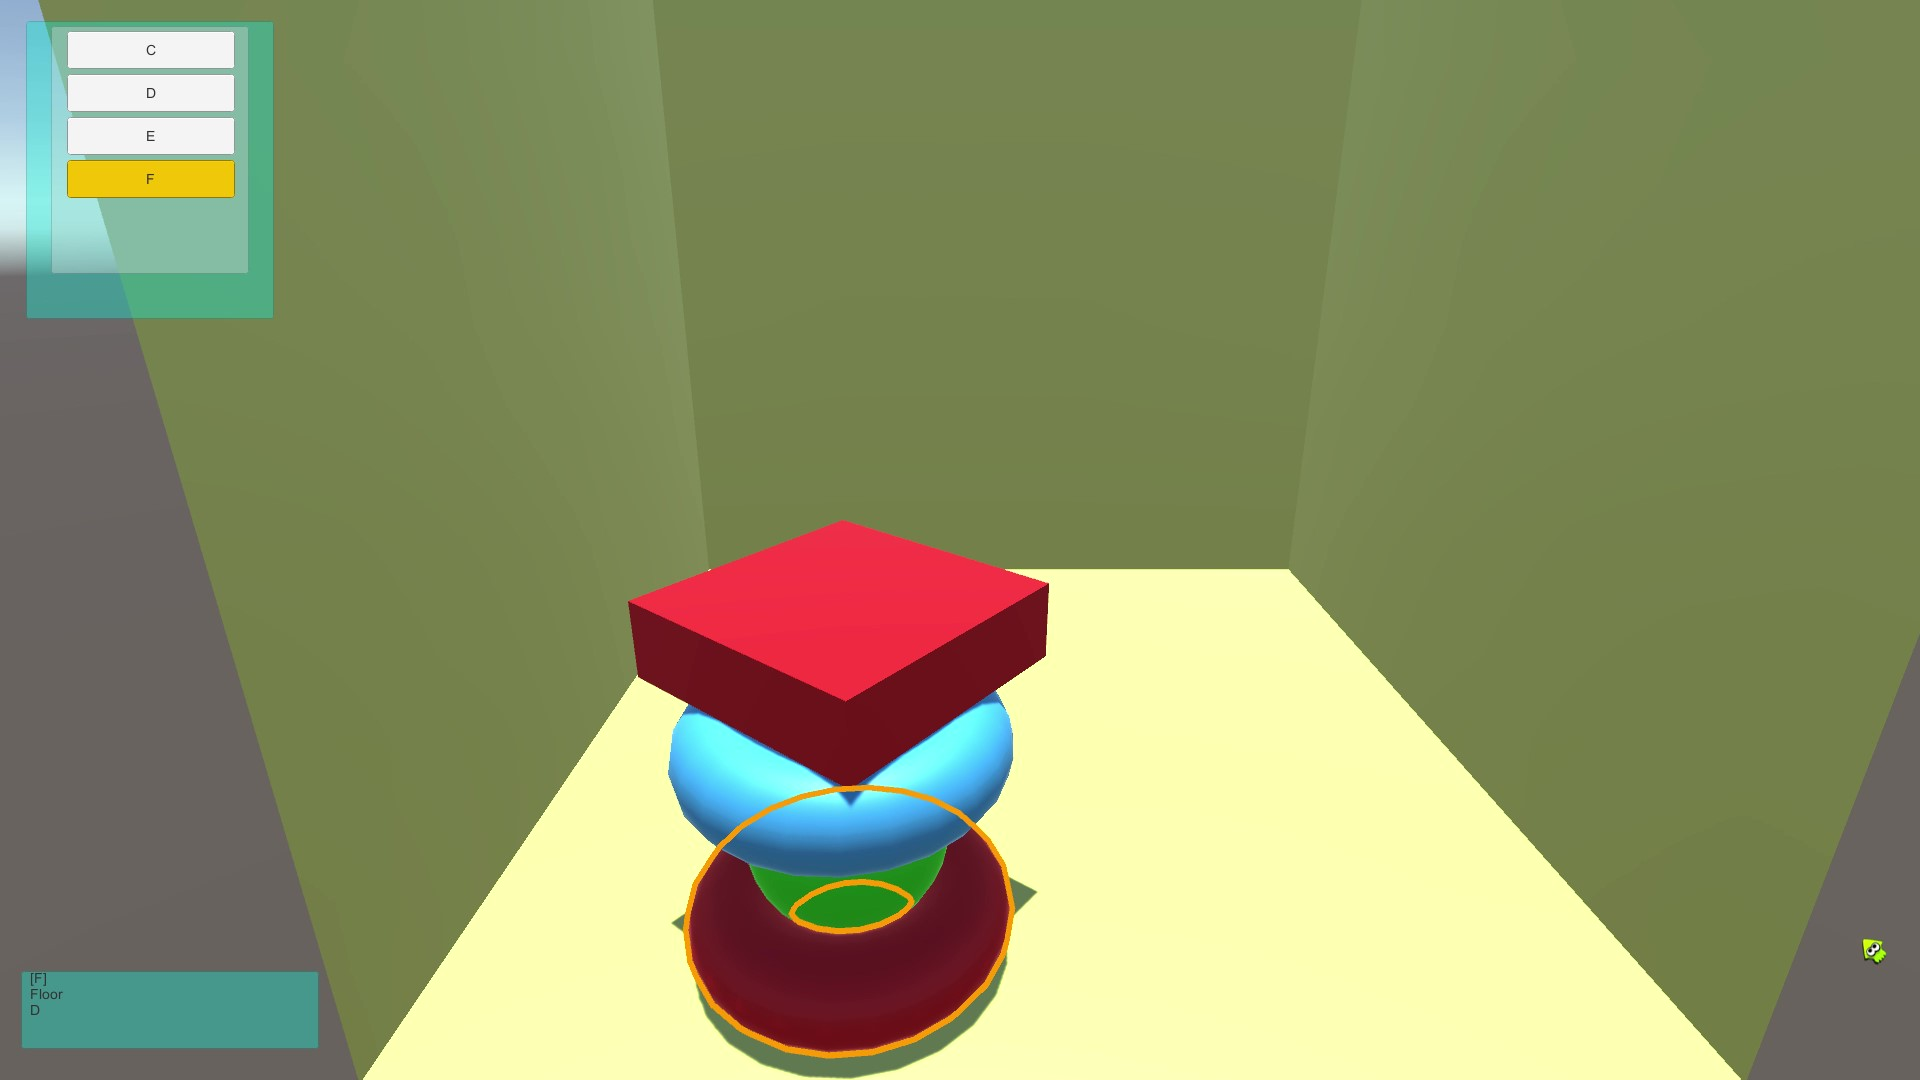
\includegraphics[scale=0.2]{images/BWP_Work6/bwp10.jpg}
  		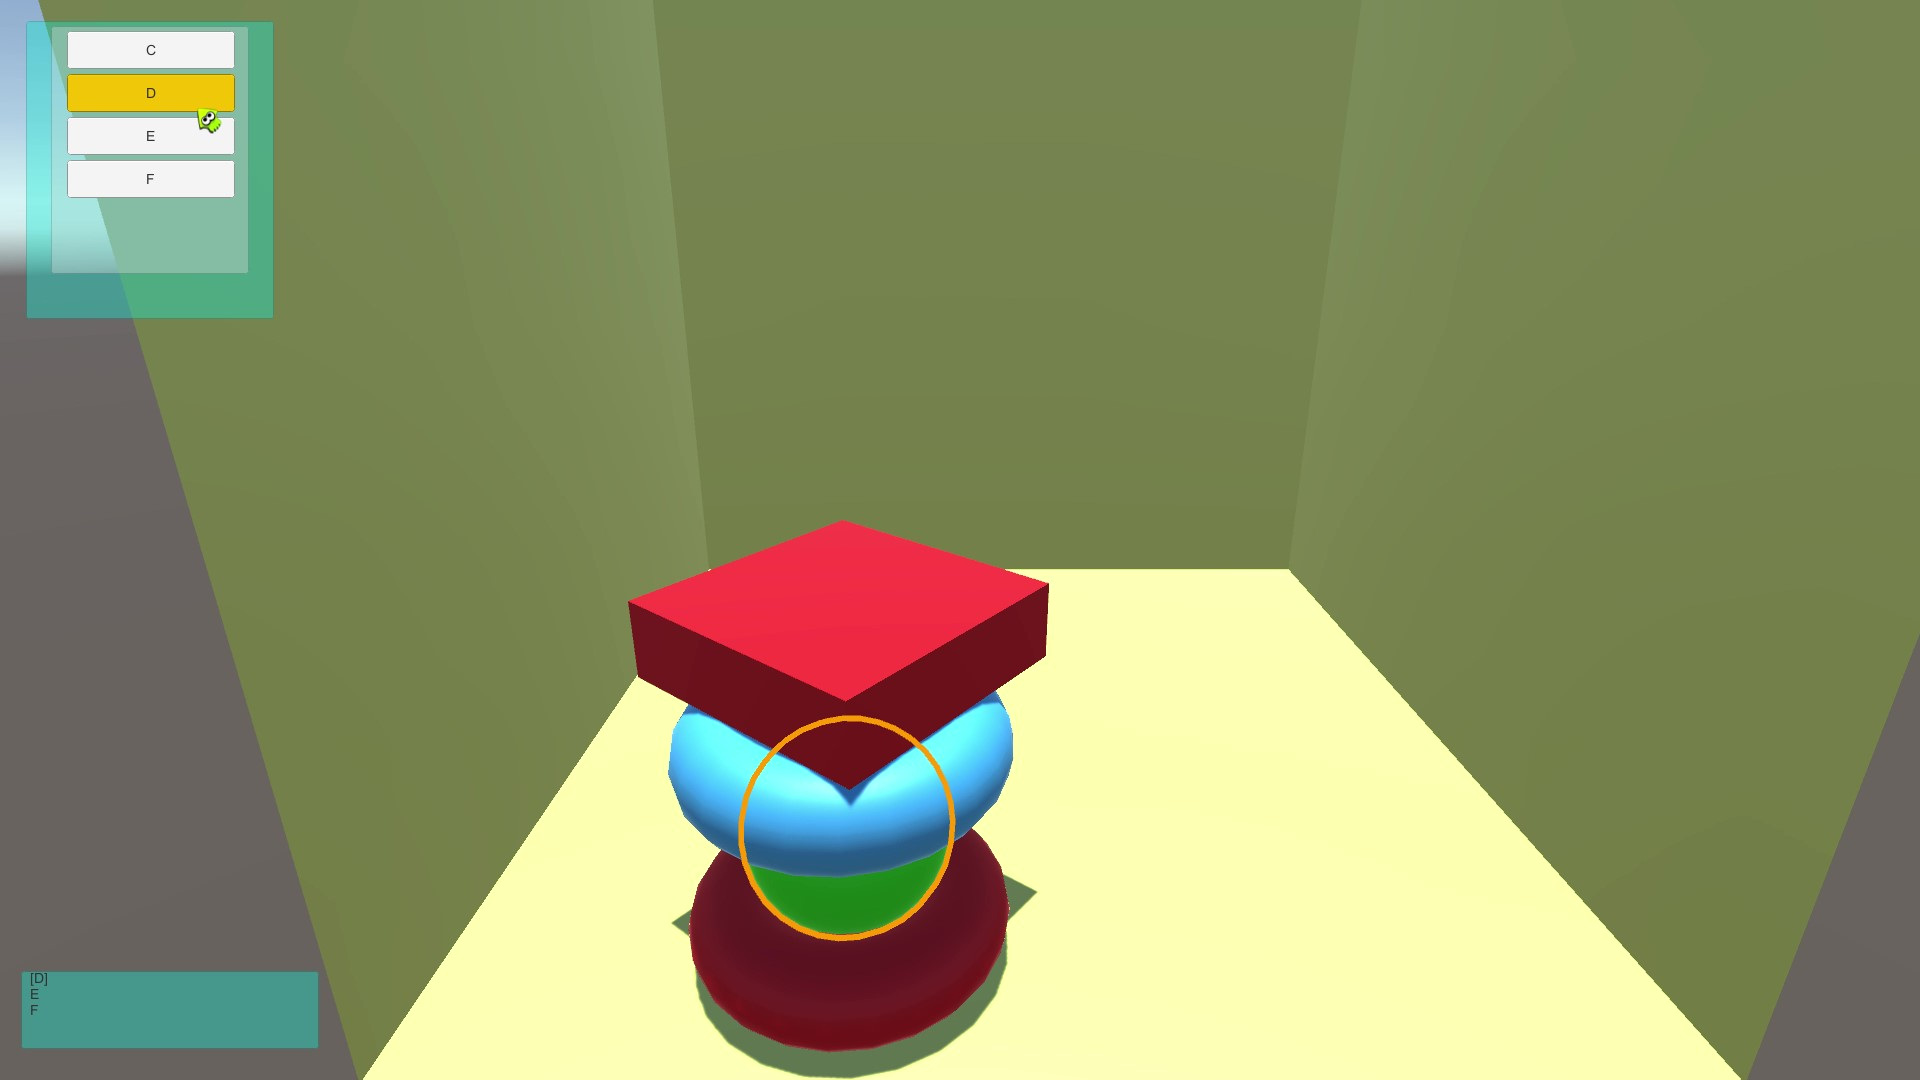
\includegraphics[scale=0.2]{images/BWP_Work6/bwp11.jpg}
	\end{center}
  	\caption{プランニング完了時の各ブロックの衝突情報}
  	\label{fig:run7}
\end{figure}
\clearpage

\subsection{考察}
Generatorスクリプト(ソースコード\ref{src:gen})にて,switchを用いているが,ここで用いる変数objの宣言の際,初期化しないとコンパイルエラーになることはC\#の特徴として挙げられると考えられる.

GUIを実装し始めた際,自動で追加されたEventSystemというオブジェクトを誤って消してしまい,実行してもButtonやInputFieldが全く反応しないという事態に陥った.EventSystemを追加し直すことで修正できたが,このように自動で用意されるものに甘んじて各種機能を使うことは,便利な反面で,何かトラブルが起こったときに簡単には自力で直せないという事態が起こり得ることに繋がるため,自分が利用している機能はどのようなものに基づいてどのように動いているのかを探求することは,今後それを用いてより高度なことをするときのためにも大切なことだと感じた. \\

uGUIでのGUI実装とSwingでのGUIの実装と比較してみると,Swingよりも並列動作は扱いやすく,Swingよりも変数の管理は面倒だと感じた.UnityでのGUIの部品となる各オブジェクトは,常時独立して動き続けているため,並列的な動作を行ったときにどのような挙動をとるかをオブジェクト毎に確認できるため挙動の管理がしやすいのだと考えられる.一方で,各オブジェクトが独立しているということは,オブジェクト間の変数はスクリプトを用意して共有する必要があるということなので,並列動作の分かりやすさと変数の管理の楽さはトレードオフの関係にあることが考えられる.

また,uGUIとSwingのいずれも,フォーカスの操作はとっつき辛いと感じた.しかし,uGUIではGUI全体のフォーカスが1つのEventSystemによって明確に行われているため,その点ではuGUIの方が把握しやすいと感じた.

しかし,GUIの一番の難点は,やはり実行する環境によって表示のされ方が異なってくることだと考えられる.その点では,Swingも標準の機能としてレイアウトが用意されてはいるが,uGUIでのアンカーを用いた配置の方が,断然とっつきやすく,調整もしやすいと感じた.

以上のことから,今後GUIを作る際は,基本的にSwingよりもuGUIで良いと考えられる.しかし,軽量化という点においてuGUIはSwingに優ることができるか,または優る必要があるかということは今後の課題である. \\

Unityを使って一番悩まされたことが,プレハブにアタッチしたコンポーネントの変数がpublicでも,その変数に他のオブジェクトを直接アタッチして参照させることができなかったことである.そのため,GameObject.Findメソッドで毎度目的のオブジェクトを探して参照を作っているが,直接アタッチできる方が効率的だと考えられる.前回も,通常のオブジェクトだと上手くいくのにプレハブだとうまくいかないようなこと(Torusの衝突判定)があったように,ブレハブの特性や注意点で理解できていないことがまだ多々あることが考えられる.Unityを使っていく上でプレハブは欠かせない機能なので,今後も積極的に使って学んでゆきたい.

また,Unityではオブジェクトを消去するという機能があるため,この点も注意して使っていかなければいけないと考えられる.Unityに限らず並列処理を行うようなプログラムでは,先程まで参照していたものが突然なくなるということが往々にして起こり得るため,その点も留意した上でのプログラム実装を行ってゆく必要があると考えられる.

また,Unityにおいて,変数をオブジェクト間で共有するために,いちいちスクリプトを作成する必要があると述べたが,共有する変数ごとにスクリプトを作成するのではなく,共有すべき変数をまとめて管理するようなスクリプトと,そのためのオブジェクトを作成して,そこを共有変数の仲介場所とすると改善できることが考えられる.例えば,今回のプログラムではStaterがその仲介場所として適していたと考えられる.更に,Staterを仲介場所にすればステータスの表示もより自在に行えるようになることが考えられ,一石二鳥である.また,このような方法で共有する変数を管理したほうが,プログラムの保守性的にも良いということが考えられる. \\

今回の実装について,開始時点を決めれるようにしたことで,初期状態の明確化ができるようになった.

最終的に自動でのプランニングを実装するには,その前段階として実装する必要のあるものが多くあったため,その過程の一部を実装しようと思い今回作ったような実装となった.
ブロックの属性付与や生成したブロックの管理,衝突情報の管理が行えるようにしたことで,プランニング実装に向けて次に必要なのは,衝突情報を突き詰め,どちらのブロックが上に乗っているかといった相対的な位置関係の取得・管理をすることと,それに基づきどの物体を目標状態に向けてどう動かすかを選択することの実装だと考えられる.
しかし,3次元空間における物体間の衝突の仕方は多様であり,どちらのブロックが上に乗っているかを厳密に判別することは困難な場合が多く存在することが考えられる.また,それを解決したところで,物体を動かすことによる状態変化も不定であり,目標状態に向けた行動の選択を一意的に決めることは難しいと考えられる.このように,実装上の難しさだけでなく,そもそも3次元空間上においてどのようにプランニングを定義するかという実世界的な難しさが数多くあることを改めて痛感した.

\section{感想}

アウトラインの実装にあたって,今回は既存のアセットを導入して実装したが,初めは自分でアウトラインのシェーダを作ることでの実装を試みていた.しかし,Shaderもそれ自体が1つの言語であるように奥深く,思ったとおりに実装することは難しかった.自在に物体を彩るのには欠かせない知識であるため,いずれシェーダについても勉強してみたいと思う.

これまでLaTeXでレポートを書いてきたが,相互参照が文字化けすることが多くあった.しかし,タイプセットを2回すれば解決できる\cite{latex}ということが知れて,嬉しかった.

この講義全体を振り返り,GUIを作る能力や,チームで協力して1つのプログラムを作る能力,GitHubやSlackやLaTeXを使う能力を大きく向上することができたと感じている.特に,これまでチームでプログラムを作ることに苦手意識があったため,この経験を今後にも活かしてゆきたいと思う.

また,チームメンバーにも非常に恵まれていたと思う.互いに支え合い,高め合うことができた.この縁も大切にし,今後にも繋げてゆきたい.

% 参考文献
\begin{thebibliography}{99}
\bibitem{unity} Unity Technologies.: 『Unity - Manual: Unity User Manual (2019.2)』 https://docs.unity3d.com/Manual/index.html (2020/01/06アクセス)
\bibitem{ugui} 竹内 大五郎: 『uGUIチュートリアル - Metal Brage』 http://www.metalbrage.com/UnityTutorials/uGUI/index.html (2020/01/06アクセス) \\
\bibitem{sv} shimoaraiso: 『UnityのScrollViewで一覧表示を作成する』 https://tech.pjin.jp/blog/2016/08/30/unity\_skill\_3/ (2020/01/06アクセス) \\
\bibitem{outline} chrisnolet: 『chrisnolet/QuickOutline: Unity asset for adding outlines to game objects』 https://github.com/chrisnolet/QuickOutline (2020/01/06アクセス) \\
\bibitem{sb} hiyotama: 『【Unity開発】uGUIのScrollbarの使い方【ひよこエッセンス】 - Unity(C\#)初心者・入門者向けチュートリアル ひよこのたまご』 https://hiyotama.hatenablog.com/entry/2015/07/04/090000 (2020/01/06アクセス) \\
\bibitem{latex} PukiWiki Developers Team.: 『【LaTeX入門/相互参照とリンク - TeX Wiki』 https://texwiki.texjp.org/?LaTeX?LaTeX入門\%2F相互参照とリンク\#h84e81eb (2020/01/06アクセス) \\
\end{thebibliography}

\end{document}
